% Semantic attack-space motivation, followed by two examples from other settings.
\begin{tikzpicture}[remember picture,overlay,
 every node/.style={text=Ink,align=center,inner sep=0pt}]
\begin{scope}[shift={(current page.south west)}]
 \node[anchor=west,font=\normalsize] at (.65,7.0)
  {The attack space is \textbf{semantically defined} \detail{(among many others)}};
 \node[anchor=west,font=\normalsize] at (.65,6.42)
  {Appealing defenses from other settings \textbf{don't transfer over}};
 \draw[Muted!35,line width=.5pt] (.65,5.94)--(15.35,5.94);
 \node[font=\normalsize\bfseries] at (4.2,5.4) {Convex outer bounds};
 \node[font=\normalsize\bfseries] at (11.85,5.4) {Randomized smoothing};
 \node[font=\fontsize{7.5}{9}\selectfont,text=Muted] at (11.85,5.02)
  {\href{https://jailbreak-tutorial.github.io/}{Image from Hassani et al., 2025}};
 \node at (4.2,3.52)
  {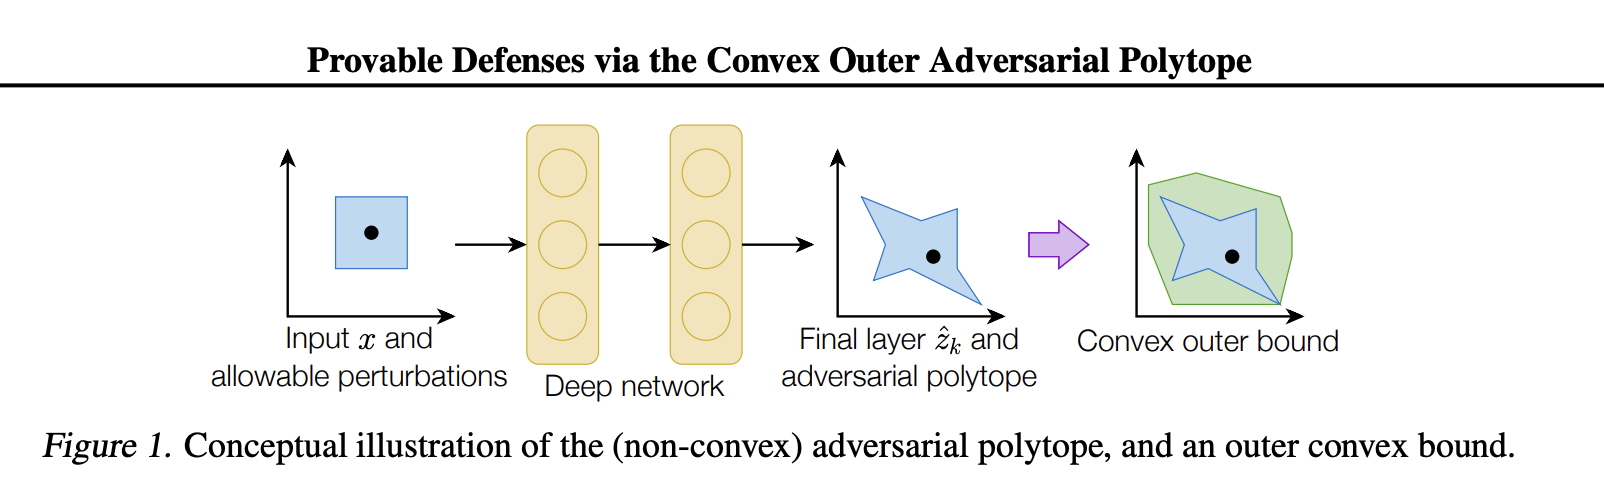
\includegraphics[width=7.1cm,
   trim=185bp 70bp 250bp 115bp,clip]{assets/convex-polytope.png}};
 \node at (11.85,3.52)
  {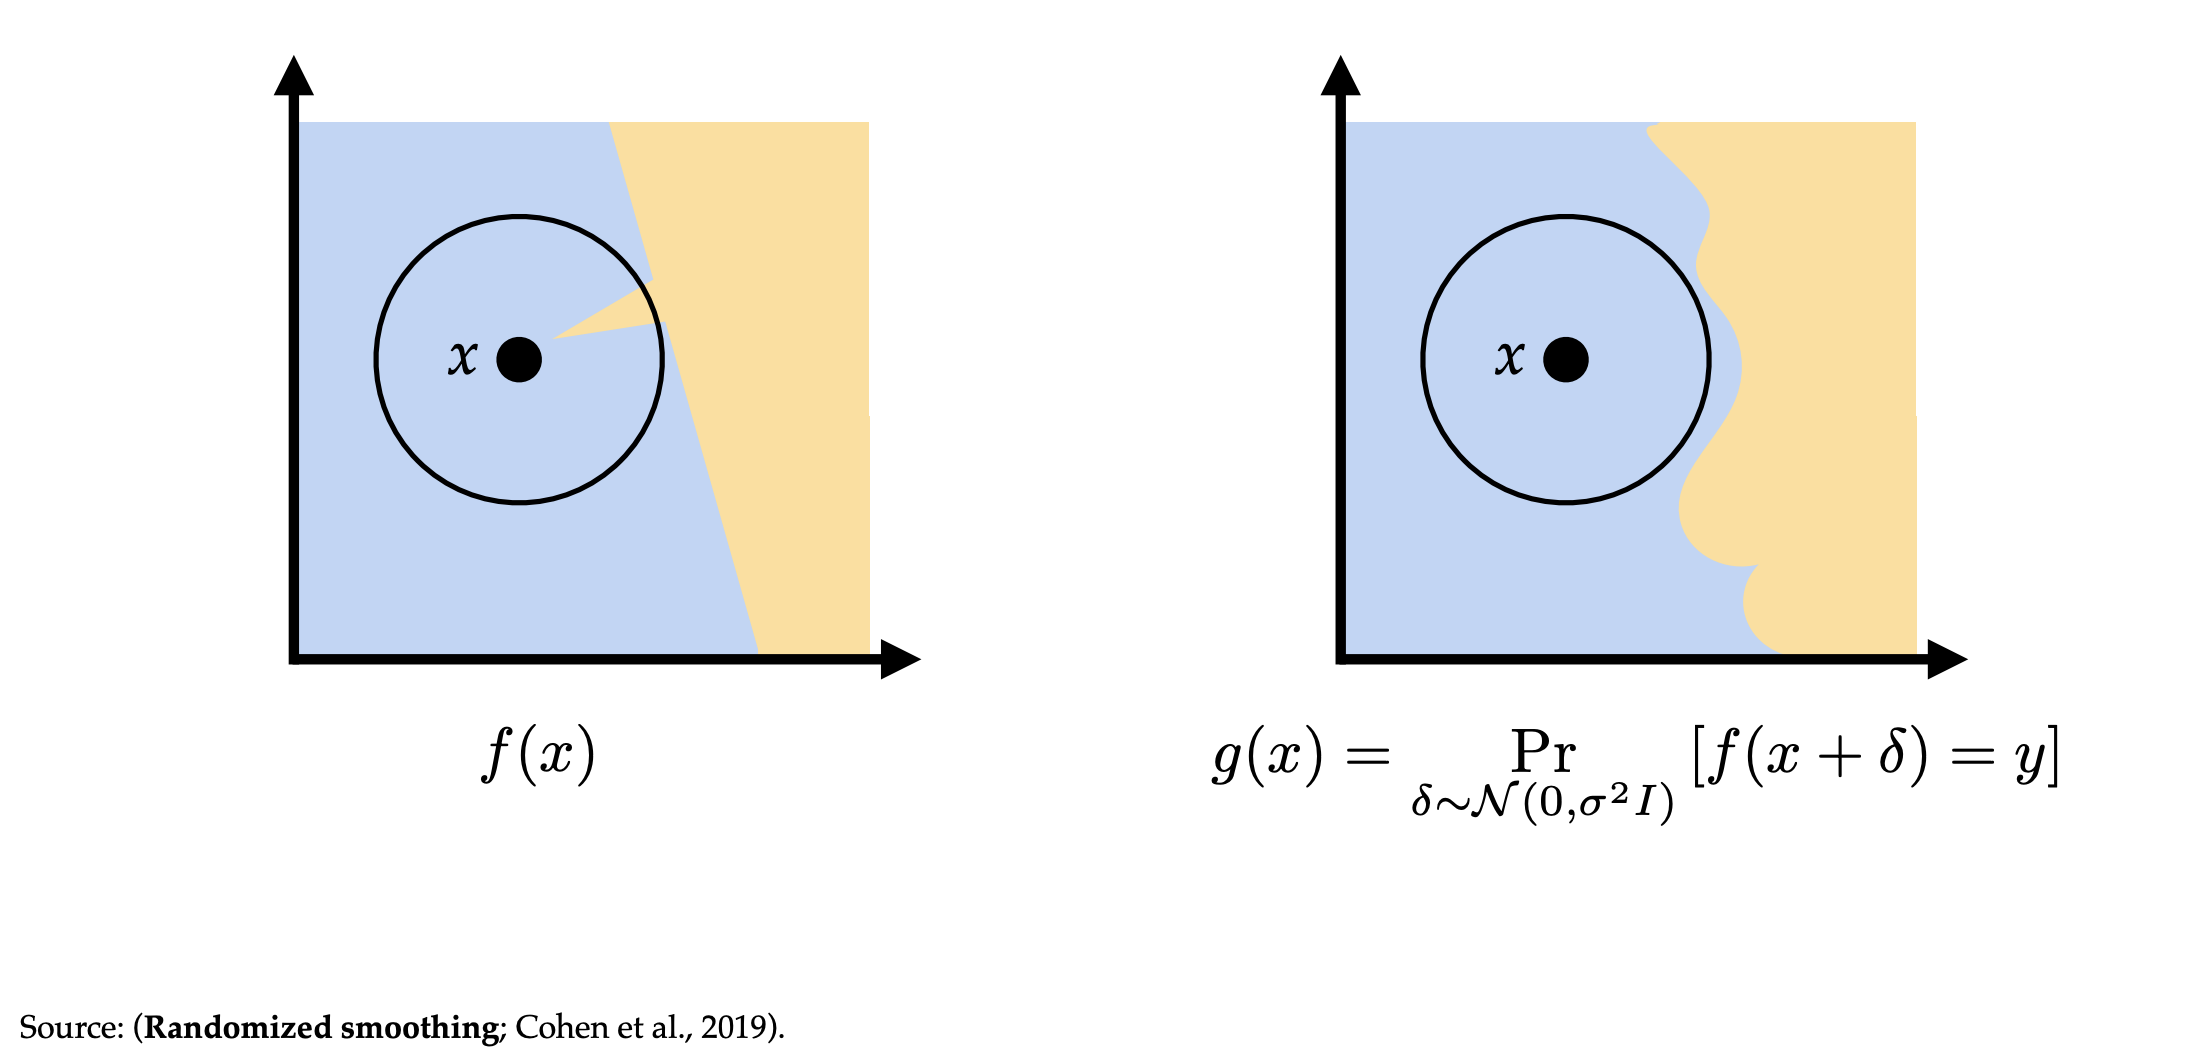
\includegraphics[width=6.1cm,
   trim=130bp 110bp 50bp 20bp,clip]{assets/randomized-smoothing.png}};
 \node[anchor=north west,align=left,font=\referencefont,text=Muted] (convex-title) at (.65,1.92)
  {\textit{Provable Defenses against Adversarial Examples}};
 \node[anchor=north west,align=left,font=\referencefont,text=Muted] at ([yshift=-.06cm]convex-title.south west)
  {Wong and Kolter, ICML 2018};
 \node[anchor=north west,align=left,font=\referencefont,text=Muted] (smoothing-title) at (8.35,1.92)
  {\textit{Certified Robustness via Randomized Smoothing}};
 \node[anchor=north west,align=left,font=\referencefont,text=Muted] at ([yshift=-.06cm]smoothing-title.south west)
  {Cohen, Rosenfeld, Kolter, ICML 2019};
\end{scope}
\end{tikzpicture}
